\section{Выполнение работы}
\subsection{Описание тестового стенда}
Для выполнения работы использовалось два тестовых стенда:
\begin{itemize}
\item Платформа Raspberry Pi 1 с ОС ArchLinux и модуль SIM-808
\item Компьютер с ОС Ubuntu 16.04
\end{itemize}

В реальном стенде будет использована плата Raspberry Pi Zero и сим модуль SIM-808L. А благодаря тому, что модуль SIM-808 полностью совместим с модулем SIM-808L, то демон, который был разработан с использованием одного модуля будет совместим с другим модулем. Так как демон создавался независимым от реализации платформы, то не имеет особого значения, на какой ОС вести разработку.

\subsection{Выбор библиотеки}
Как было рассмотренно, для реализации общения по D-Bus существует несколько различных библиотек. Исходя из проведенного анализа, была выбрана библиотека \textit{dbus-glib} по той причине, что используемое устройствоя является маломощным, а так как у выбранной библиотеки малый уровень абстракции, то данный выбор позволяет нам увеличить производительность.

\subsection{Разработка демона}
Исходный код демона приведен в листинге \ref{lst:main}. В основной функции приложения main производятся следующие действия:
\begin{itemize}
\item Запись в лог информации о старте демона 
\item Подключение к системной шине D-Bus
\item Получение списка доступных модемов
\item Выбор модема
\item Попытка активации модема
\item Получение оператора
\end{itemize}

Парсинг полученного ответа и запись в лог-файл осуществляется с помощью заголовочного файла, код которого приведен в листинге \ref{lst:struct}. В данном заголовочном файле реализована структура, которая соответствует большинству ответов. В структуре два поля:
\begin{itemize}
\item Строка, соответствующая пути оьъекта (например, \textit{/sim900\_0} --- путь используемого модуля).
\item Словарь, который соответствует свойствам, где ключ - свойство, а значение - значение свойства.
\end{itemize}

Также, в демоне реализовано подключение к сигналу и его обработка. Далее будет подробнее рассмотрен этап подключения к сигналу.
\begin{itemize}
\item \textit{dbus\_error\_init} производит инициализацию структуры ошибки D-Bus.
\item \textit{dbus\_bus\_get} подключение к системной шине D-Bus.
\item \textit{dbus\_error\_is\_set} проверка на возникновение ошибки D-Bus.
\item \textit{dbus\_connection\_setup\_with\_g\_main} устанавливает функции наблюдения и тайм-аута DBusConnection для интеграции соединения с основным циклом.
\item \textit{dbus\_bus\_add\_match} добавляет правило соответствия для сообщений, проходящих через шину.
\item \texttt{dbus\_connection\_add\_filter} дообавляет фильтрпацию сообщений. Фильтры --- это обработчики сообщений, которые вызываются для обработки всех входящих сообщений, относящихся к зарегистрированному объекту. 
\end{itemize}

Помимо файла с исходным кодом и заголовочного файла, в структуру проекта входит \textit{CMakeLists} --- файл, предназначенный для сборки проекта. Содержание данного файла приведено в листинге \ref{lst:cmake}.

Пример исправной работы демона можно увидеть на рис. \ref{fig:daemon}

\begin{figure}
\center{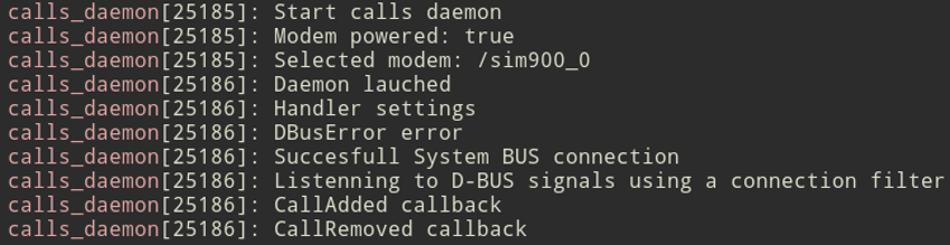
\includegraphics[width=0.6\linewidth]{daemon}}
\caption{Пример исправной работы демона}
\label{fig:daemon}
\end{figure}

\section{Дополнительная работа}
В ходе проекта, помимо создания демона звонков, была создана графическая оболочка для приложения телефона. В качестве платформы для создания графических приложений рассматривались две, одна из которых была описана выше, --- \textit{Qt} и \textit{GTK+}. В конечном итоге, была выбрана платформа Qt из-за того, что графика, написанная на \textit{Qt}, на конечной платформе выглядит приятнее, чем графика, написанная на \textit{GTK+}. 

Для создания графической оболочки была использована связка \textit{QT + QML}, а основная логика приложения --- \textit{C++}. Самым первым этапом создания основной логики приложения является создание самого приложения \textit{QApplication} (Листинг \ref{lst:mainqt}).
\begin{lstlisting}[label=lst:mainqt, caption={Создание приложения}]
int main(int argc, char *argv[])
{
	QApplication a(argc, argv);
	MainWindow w;
	return a.exec();
}
\end{lstlisting}
Класс \textit{MainWindow} представляет из себя основную логику графического окна. Реализация данного класса приведена в листингах~\ref{lst:mainwindowgui} --- \ref{lst:mainwindowh}. В данном классе выполняются следующия действия:
\begin{itemize}
\item Подключение к созданному приложению графической оболочки
\item Получение активированного модема
\item Совершение вызова
\item Завершение вызова
\end{itemize}

Для подключения графической состовляющей и различных изображений используются ресурсы. Использование ресурсов позволяет облегчить сборку приложения, тем самым, платформа нагружается немногим меньше, а время сборки уменьшается. Файл ресурсов выглядит следующим образом (листинг~\ref{lst:res}).
\begin{lstlisting}[label=lst:res, caption={Файл ресурсов}]
<RCC>
	<qresource prefix="/">
		<file>qml/main.qml</file>
		<file>qml/dialing.qml</file>
		<file>qml/core/Button.qml</file>
		<file>qml/call.qml</file>
		<file>pics/dial.png</file>
		<file>pics/erase.png</file>
		<file>pics/back.png</file>
		<file>pics/hang.png</file>
	</qresource>
</RCC>
\end{lstlisting}

Окна с графической реализацией имеют расширение \textit{.qml}. Главное окно и реализация класса \textit{Button} приведены в листингах~\ref{lst:mainqml}---\ref{lst:button}. Так как вместо стандартного класса \textit{Button} был использован свой класс, то приложению необходимо сообщить о том, что когда программист пытается реализовать класс \textit{Button}, вместо стандартного, нужно реализовывать созданный. Для этого нужна всего одна строчка в файле \textit{qmldir} (Листинг~\ref{lst:qmldir}).
\begin{lstlisting}[label=lst:qmldir, caption={Подключение класса Button}]
Button Button.qml
\end{lstlisting}

Для сборки проекта написанного на Qt принято использовать утилиту \textit{qmake}. Для ее использования создается файл с расширением \textit{.pro} и в него прописываются все зависимости. Используемый файл \textit{phone.pro} показан в листинге~\ref{lst:phone}.

Таким образом, было написано графическое приложение, позволяющее:
\begin{itemize}
\item Набирать номер
\item Совершать звонок
\item Отображать звонок
\item Сбрасывать звонок
\end{itemize}
Пример приложения приведен на рисунке~\ref{fig:phone}.
\begin{figure}
\center{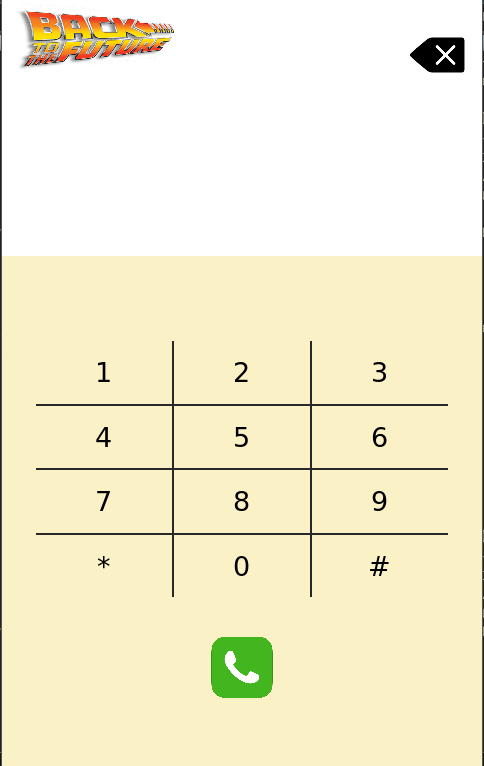
\includegraphics[width=0.6\linewidth]{phone}}
\caption{Пример работы графического приложения}
\label{fig:phone}
\end{figure}
